\documentclass[conference]{IEEEtran} % Use IEEE conference template class

% === PACKAGES ===
% IEEEtran class handles many formatting aspects automatically.
% Add essential packages not included by default.
\usepackage[utf8]{inputenc}      % Handle UTF-8 encoding
\usepackage[T1]{fontenc}         % Use modern font encodings
\usepackage{graphicx}            % For including images (\graphicspath can be useful)
\usepackage{amsmath}             % For math environments
\usepackage{booktabs}            % For professional-looking tables (\toprule, \midrule, \bottomrule)
\usepackage{url}                 % For typesetting URLs
\usepackage{cite}                % Handles citation ranges better for IEEE style
\usepackage[binary-units=true]{siunitx} % For consistent units (optional but good practice)

% Add hyperref last for best compatibility (optional)
\usepackage[hidelinks]{hyperref} % Use hidelinks to avoid boxes around links, common in IEEE papers
\hypersetup{
    colorlinks=false, % Set to false for final submission usually
    pdftitle={CNN Performance Comparison},
    pdfauthor={Geetika Khanna, Archit Harsh},
    pdfsubject={Deep Learning Performance Analysis},
    pdfkeywords={CNN, PyTorch, Numba, CUDA, MPS, CPU, GPU, Performance Benchmark, MNIST}
}

% Define graphic path (optional, helps organize images)
% \graphicspath{{results/}} % Assumes figures are in a 'results' subdirectory

% Correct bad hyphenation here
\hyphenation{op-tical net-works semi-conduc-tor Numba Py-Torch}

% === DOCUMENT START ===
\begin{document}

% === TITLE SECTION ===
\title{Convolution Neural Network Performance Analysis: CPU-optimized vs GPU-optimized}

% Author Information (Use IEEEtran format)
\author{\IEEEauthorblockN{Geetika Khanna, Archit Harsh}
\IEEEauthorblockA{Group 6\\
University of Maryland}
}

% Make the title area
\maketitle

% === ABSTRACT ===
\begin{abstract}
    The performance of deep learning models, particularly Convolutional Neural Networks (CNNs), is critically dependent on the underlying hardware architecture and software optimization strategies. This paper presents a comparative performance analysis of a standard CNN architecture trained for image classification on the MNIST dataset. We implement and evaluate the CNN using five distinct execution backends: 
    \begin{enumerate}
        \item A multi-core CPU optimized using Numba's Just-In-Time (JIT) compilation,
        \item an NVIDIA GPU accelerated via Numba's CUDA JIT,
        \item a multi-core CPU utilizing the standard PyTorch framework,
        \item an NVIDIA GPU accelerated via PyTorch's CUDA backend, and
        \item an Apple Silicon GPU utilizing PyTorch's Metal Performance Shaders (MPS) backend.
    \end{enumerate}
    We analyze the performance of each implementation in terms of training time per epoch, overall training throughput, final test accuracy, and basic memory usage (RAM/VRAM). The results provide empirical insights into the speedup potential, resource utilization, and characteristics of each hardware acceleration approach and framework choice for this common CNN workload. The complete source code is available on GitHub: \url{https://github.com/geetikak13/cnn_performance_comparison}.
\end{abstract}

% === SECTIONS ===

\section{Introduction}
\label{sec:introduction}
Convolutional Neural Networks (CNNs) have become fundamental tools in computer vision, achieving state-of-the-art results in tasks like image classification \cite{Krizhevsky2012}. However, training these complex models is computationally intensive, often requiring significant processing power and time \cite{Sze2017}. This computational demand has driven the adoption of hardware accelerators, primarily Graphics Processing Units (GPUs), to make deep learning training feasible \cite{Krizhevsky2012}.

While NVIDIA's CUDA platform has traditionally dominated GPU acceleration, the landscape is evolving. Apple's Silicon processors, featuring integrated GPUs with the Metal Performance Shaders (MPS) framework, offer a compelling alternative within the macOS ecosystem \cite{Hubner2025}. Concurrently, optimizing performance on traditional multi-core Central Processing Units (CPUs) remains crucial, especially for inference deployment, smaller models, or environments without dedicated GPUs. Furthermore, the choice of programming framework significantly influences both performance and developer productivity. High-level frameworks like PyTorch provide extensive pre-optimized operations and automatic differentiation, while lower-level tools like Numba offer fine-grained control via Just-In-Time (JIT) compilation for CPU and CUDA targets.

This project undertakes a direct performance comparison across these diverse hardware and software combinations. We investigate the practical performance trade-offs by implementing and benchmarking a standard CNN architecture for the MNIST handwritten digit classification task \cite{LeCun1998} using five distinct approaches: Numba on CPU, Numba on CUDA, PyTorch on CPU, PyTorch on CUDA, and PyTorch on MPS. The primary objectives are to:
\begin{itemize}
    \item Quantify the speedup achieved by different GPU acceleration methods (Numba CUDA, PyTorch CUDA, PyTorch MPS) compared to CPU execution (Numba CPU, PyTorch CPU).
    \item Compare the performance of Numba and PyTorch implementations on the same hardware (CPU and CUDA).
    \item Evaluate the performance characteristics (speed, throughput, accuracy, memory usage) of each platform.
    \item Provide empirical data to inform decisions regarding hardware and framework selection for similar CNN workloads.
\end{itemize}
The significance of this work lies in providing a practical, head-to-head comparison using contemporary tools on a common benchmark task, offering insights relevant to researchers and practitioners navigating the diverse landscape of deep learning acceleration.

\section{Literature Survey}
\label{sec:literature}
The field of hardware acceleration for deep learning is well-established. The seminal work by Krizhevsky et al. \cite{Krizhevsky2012} demonstrated the transformative impact of GPU acceleration (using CUDA) on training deep CNNs, enabling breakthroughs in image classification accuracy on datasets like ImageNet. Sze et al. \cite{Sze2017} provide a comprehensive tutorial and survey covering various hardware optimization techniques. Their work discusses both CPU-level strategies, such as vectorization through SIMD (Single Instruction, Multiple Data) instructions leveraged by libraries like Intel MKL or OpenBLAS (which Numba and PyTorch's CPU backend can utilize), and the principles of GPU parallelism that make GPUs effective for the matrix and tensor operations inherent in CNNs.

Several studies have compared different deep learning frameworks, often focusing on high-level APIs like TensorFlow versus PyTorch on specific hardware (typically CPU or NVIDIA GPUs). However, comparisons involving lower-level JIT compilation tools like Numba, which allow for Python-based custom kernel development, are less common, especially across multiple hardware targets (CPU and CUDA). Numba provides a way to achieve C-like performance from Python code for numerical tasks, making it an interesting alternative for performance-critical components or custom operations not readily available in high-level frameworks.

The advent of Apple Silicon has spurred research into its capabilities for scientific computing and machine learning. Hubner et al. \cite{Hubner2025} evaluated the performance and energy efficiency of Apple's M-series SoCs, highlighting the potential of the integrated GPU and the MPS framework. While MPS aims to provide optimized primitives for common machine learning operations, its performance relative to established CUDA implementations on comparable hardware tiers is an area of active interest.

Our project builds upon this existing work by focusing specifically on a direct comparison involving both Numba (for CPU and CUDA) and PyTorch (for CPU, CUDA, and MPS) for the same CNN task. We selected these tools for their relevance to the Python data science ecosystem and their representation of different levels of abstraction in utilizing hardware acceleration. This allows us to evaluate not only hardware performance but also the implications of framework choice on development and execution speed.

\section{Methodology}
\label{sec:methodology}
This section details the dataset, model architecture, specific implementation approaches for each platform, tools, hardware used, and the optional containerization strategy.

\subsection{Dataset}
We utilized the standard MNIST dataset of handwritten digits \cite{LeCun1998}. It consists of 60,000 28x28 pixel grayscale training images and 10,000 test images, representing digits 0 through 9.
\subsubsection{Preprocessing} Pixel values were normalized from the original [0, 255] range to [0.0, 1.0] by dividing by 255.0. For the PyTorch implementations, an additional normalization step using the dataset's mean (0.1307) and standard deviation (0.3081) was applied via `torchvision.transforms`.
\subsubsection{Padding} To ensure consistent batch processing and avoid handling partial batches, both the training and test sets were padded. If the number of samples was not an exact multiple of the batch size (default 512), samples were repeated from the beginning of the respective dataset until the total count was divisible by the batch size. This padding was handled within the data loading functions (`data/preprocess.py`) for both NumPy and PyTorch data loaders.
\subsubsection{Data Loading} For Numba implementations (CPU, CUDA), data was loaded into NumPy arrays using `tensorflow.keras.datasets.mnist` (as per the initial example code) and preprocessed. A channel dimension was added, resulting in shapes like (N, 1, 28, 28). For PyTorch implementations (CPU, CUDA, MPS), data was loaded using `torchvision.datasets.MNIST` and `torch.utils.data.DataLoader`, which handles batching and shuffling automatically.

\subsection{CNN Architecture}
A consistent CNN architecture was implemented across all platforms, based on the structure in the provided example code:
\begin{enumerate}
    \item \textbf{Input:} (Batch Size, 1, 28, 28)
    \item \textbf{Convolutional Layer 1:} 8 output filters, 3x3 kernel, stride 1, no padding. Followed by ReLU activation. Output shape: (Batch Size, 8, 26, 26).
    \item \textbf{Max Pooling Layer 1:} 2x2 kernel, stride 2. Output shape: (Batch Size, 8, 13, 13).
    \item \textbf{Convolutional Layer 2:} 16 output filters, 3x3 kernel, stride 1, no padding, taking 8 input channels. Followed by ReLU activation. Output shape: (Batch Size, 16, 11, 11).
    \item \textbf{Max Pooling Layer 2:} 2x2 kernel, stride 2. Output shape: (Batch Size, 16, 5, 5).
    \item \textbf{Flatten Layer:} Reshapes the output to a 1D vector. Output shape: (Batch Size, 16 * 5 * 5 = 400).
    \item \textbf{Dense Layer 1 (Hidden):} 128 output units. Followed by ReLU activation. Output shape: (Batch Size, 128).
    \item \textbf{Dense Layer 2 (Output):} 10 output units (one per MNIST class). Output shape: (Batch Size, 10). For Numba versions, an explicit Softmax activation was applied. For PyTorch versions, raw logits were output, as `nn.CrossEntropyLoss` incorporates the Softmax calculation.
\end{enumerate}
Weight initialization for dense layers used He initialization \cite{He2015}, suitable for ReLU activations. Convolutional weights used a simple scaled random initialization as per the example code.

\subsection{Implementations}
Five distinct implementations were developed:
\begin{itemize}
    \item \textbf{Numba CPU :} Core operations (convolution, pooling, dense layers, activations) were implemented as separate functions decorated with Numba's `@njit(parallel=True, cache=True)`. Data was stored in NumPy arrays. Backpropagation for the two dense layers and weight updates using SGD with momentum were implemented manually within Numba-compiled functions.
    \item \textbf{Numba CUDA :} Forward pass operations were implemented as CUDA kernels using Numba's `@cuda.jit`. Data management involved explicit transfers between CPU (host) and GPU (device) memory. Backpropagation for dense layers and weight updates were performed on the CPU after copying required data back from the GPU. Updated weights were copied back to the GPU.
    \item \textbf{PyTorch CPU :} The CNN was defined as an `nn.Module` subclass (`ConvNetPyTorch`). Standard PyTorch layers (`nn.Conv2d`, `nn.MaxPool2d`, `nn.Linear`) and activation functions (`F.relu`) were used. The model and data tensors were explicitly kept on or moved to the CPU (`torch.device('cpu')`). Training utilized PyTorch's automatic differentiation engine (`loss.backward()`) and the `torch.optim.SGD` optimizer.
    \item \textbf{PyTorch CUDA :} Identical model definition (`ConvNetPyTorch`) as the PyTorch CPU version. The model and data tensors were moved to the NVIDIA GPU using `.to('cuda')`. Training proceeded using PyTorch's autograd and optimizer, leveraging the highly optimized cuDNN library backend for CUDA operations.
    \item \textbf{PyTorch MPS :} Identical model definition (`ConvNetPyTorch`). The model and data tensors were moved to the Apple Silicon GPU using `.to('mps')`. Training utilized PyTorch's autograd and optimizer, leveraging Apple's Metal Performance Shaders via the PyTorch MPS backend.
\end{itemize}

\subsection{Tools and Frameworks}
\begin{itemize}
    \item Python (Version 3.8+)
    \item NumPy: For numerical operations and data structures in Numba implementations.
    \item Numba: For JIT compilation on CPU and CUDA.
    \item PyTorch: High-level deep learning framework for CPU, CUDA, and MPS implementations.
    \item TensorFlow: Used solely for `tf.keras.datasets.mnist` data loading, maintaining consistency with original example code.
    \item Matplotlib \& Seaborn: For plotting results.
    \item Pandas: For data analysis and manipulation of results.
    \item Psutil: For basic process RAM monitoring.
\end{itemize}

\subsection{Hardware Environment}
All experiments were conducted on the following hardware configuration:
\begin{itemize}
    \item CPU: Intel Core Ultra 7 155H (22 CPUs)
    \item NVIDIA GPU: NVIDIA GTX 4060 (8GB DDR6 VRAM) (CUDA-enabled)
    \item Apple Silicon Chip: Apple M4 Pro 16 core GPU (with Metal support)
    \item System RAM: 16 GB
    \item Operating System: macOS 15.4.1 / Windows 11
\end{itemize}

\section{Experiments}
\label{sec:experiments}
A standardized experimental procedure was followed using the main script (`main.py`) to orchestrate the training and evaluation across the selected platforms.

\subsection{Experimental Setup}
The script managed platform selection (via `--platform` argument), hyperparameter configuration (e.g., epochs, batch size), hardware availability checks, data loading, model/optimizer initialization, the training loop execution, and metric logging via `src/logger.py` to platform-specific CSV files (e.g., `results/metrics/*) in the directory specified.

\subsection{Parameter Settings}
The default parameters used for all experiments, unless overridden by command-line arguments, were:
\begin{itemize}
    \item Epochs: 10
    \item Batch Size: 512
    \item Learning Rate: 0.01
    \item SGD Momentum: 0.9
    \item CNN Architecture: As described in Section \ref{sec:methodology}.B.
\end{itemize}

\subsection{Performance Evaluation}
The primary metrics for comparison were:
\begin{itemize}
    \item \textbf{Epoch Time:} Wall-clock time taken to complete one training epoch (including forward pass, backward pass, weight update, and any data transfers).
    \item \textbf{Training Throughput:} Number of training samples processed per second during an epoch (calculated as `number of training samples / epoch time`).
    \item \textbf{Test Accuracy:} Classification accuracy achieved on the held-out test set after each training epoch.
    \item \textbf{Total Training Time:} Total wall-clock time for the entire training process (all epochs) for a given platform.
    \item \textbf{Memory Usage:} Basic monitoring of process RAM using `psutil` and peak allocated GPU VRAM (for PyTorch CUDA only) using `torch.cuda.memory\textunderscore allocated`.
\end{itemize}
These metrics were logged to separate CSV files per platform. A separate script (`evaluation/compare\textunderscore results.py`) was used post-experiment to combine these CSVs, calculate summary statistics (averages, totals, maximums), and generate comparative plots using Pandas, Matplotlib, and Seaborn.

\section{Results}
\label{sec:results}
This section presents the outcomes of the comparative performance experiments conducted across the five implemented platforms. The results are based on training the specified CNN architecture on the MNIST dataset for 10 epochs using the default hyperparameters.

% --- Referencing Table 1 ---
Table \ref{tab:results_summary} summarizes the key performance indicators aggregated over the training duration for each platform. It includes the average time per epoch, the total time required to complete 10 epochs, the average training throughput, the final test accuracy achieved after the last epoch, the maximum test accuracy observed during training, the average process RAM usage, and the maximum GPU VRAM allocated (where applicable and measured).

\begin{table*}[htbp]
    \centering
    \caption{Performance Summary Results}
    \label{tab:results_summary} 
    \renewcommand{\arraystretch}{1.1}
    \begin{tabular}{@{}lccccccc@{}} 
        \toprule
        Platform            & Avg Epoch & Total Train   & Avg Throughput    & Final Test    & Max Test  & Avg Proc  & Max GPU   \\
                            & Time (s)  & Time (s)      & (samples/s)       & Acc (\%)      & Acc (\%)  & RAM (MB)  & VRAM (MB) \\
        \midrule
        CPU (Numba)         & 2.0928    & 20.928        & 30501             & 96.33         & 97.42     & 1334.572  & 0         \\
        GPU CUDA (Numba)    & 0.9268    & 9.268         & 71758             & 96.68         & 97.56     & 1156.894  & 0         \\
        CPU PyTorch         & 11.2687   & 112.687       & 5340              & 97.57         & 98.5      & 1611.935  & 0         \\
        CUDA PyTorch        & 8.7219    & 87.219        & 6948              & 97.21         & 98.5      & 1363.258  & 16.87     \\
        MPS PyTorch         & 9.0544    & 90.544        & 6645              & 97.31         & 98.5      & 1188.246  & 0         \\
        \bottomrule
    \end{tabular}
    \vspace{0.1cm}
\end{table*}

% --- Referencing Figure 1 ---
Figure \ref{fig:results_plots} provides a visual comparison of the performance trends over the 10 training epochs. It includes plots showing: (a) Time per Epoch, (b) Training Throughput per Epoch, (c) Test Accuracy per Epoch, and (d) a bar chart comparing the overall average training throughput across all platforms.


\begin{figure*}[htbp]
    \centering
    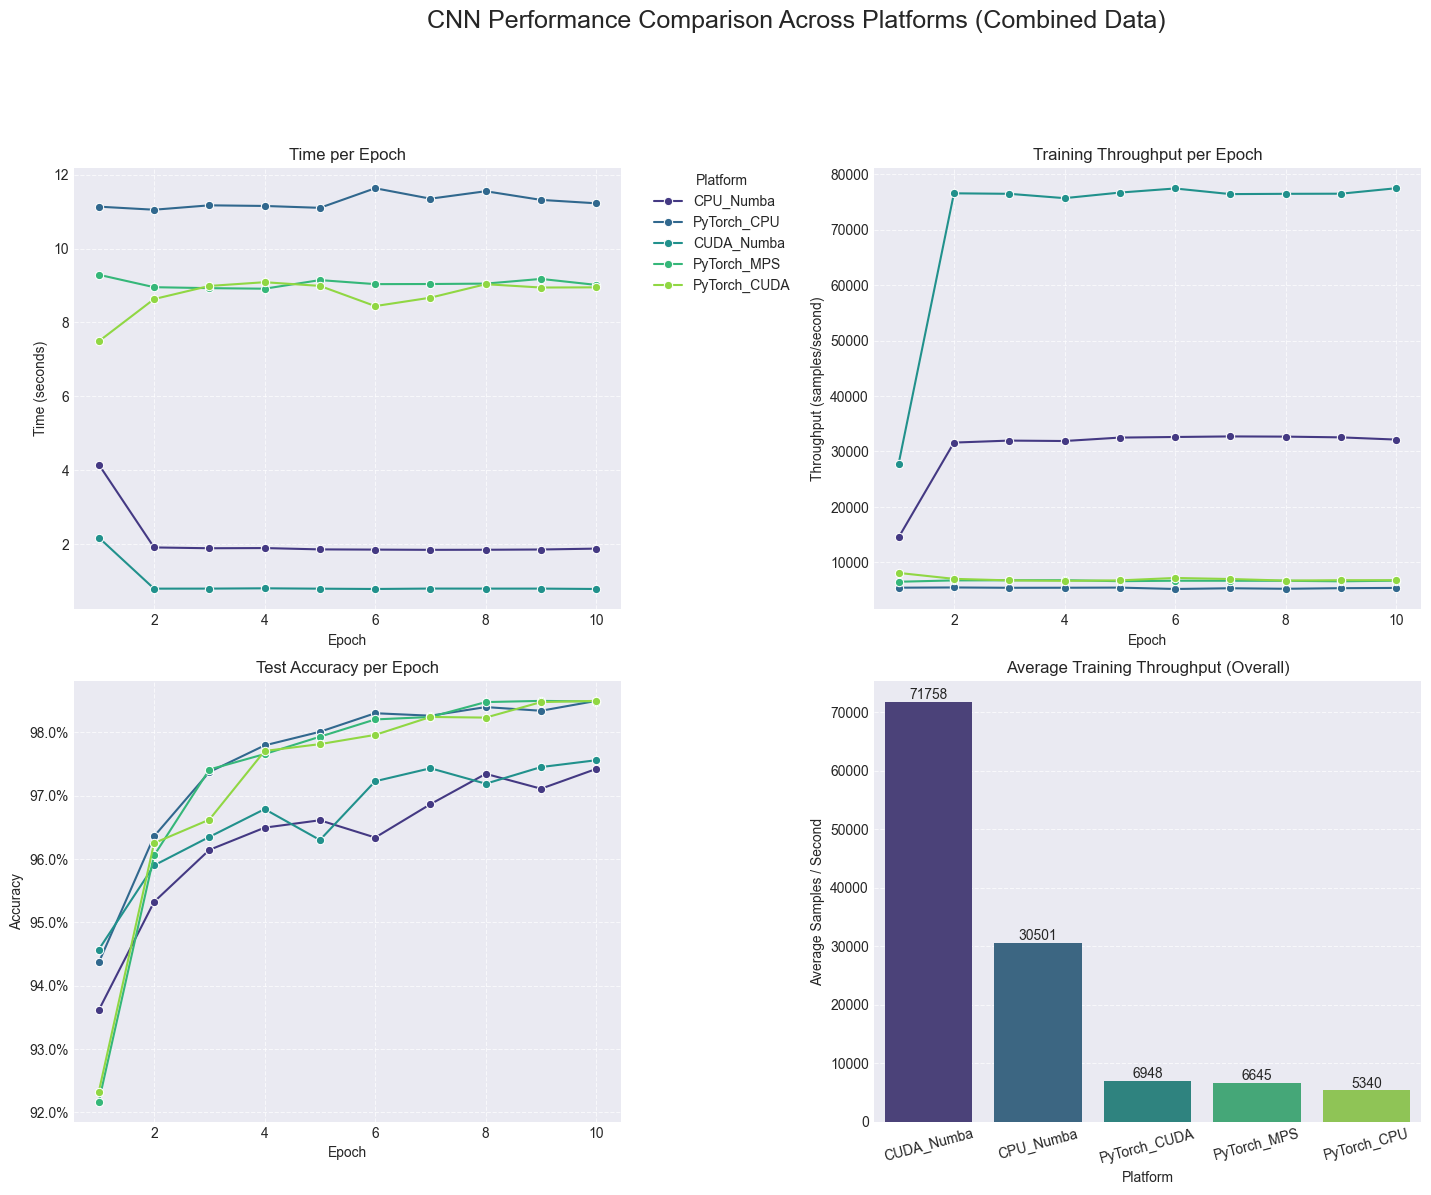
\includegraphics[width=0.98\textwidth]{results/comparison_plot_combined.png}
    \caption{CNN Performance Comparison Plots (Combined Data from all platforms)}
    \label{fig:results_plots}
    \vspace{0.1cm}
\end{figure*}

\subsection*{Analysis of Results} % Use subsection* for unnumbered analysis points
\begin{itemize}
    \item \textbf{Epoch Time:} The Numba CPU implementation was slower than Numba CUDA, taking an average of 2.09 seconds per epoch. The Numba CUDA implementation significantly reduced this to 0.93 seconds per epoch, demonstrating the effectiveness of GPU acceleration. PyTorch CPU was considerably slower than both Numba implementations, averaging 11.27 seconds per epoch, while PyTorch CUDA and MPS were faster at 8.72 and 9.05 seconds per epoch, respectively.
    \item \textbf{Training Time:} The total training time for 10 epochs was significantly lower for GPU-accelerated implementations. Numba CUDA completed in 9.27 seconds, while PyTorch CUDA and MPS took 87.22 and 90.54 seconds, respectively. In contrast, the Numba CPU and PyTorch CPU implementations took 20.93 and 112.69 seconds, respectively.
    \item \textbf{Training Throughput:} The Numba CUDA implementation achieved the highest throughput at 71,758 samples per second, followed by the Numba CPU at 30,501 samples per second. PyTorch CUDA and MPS had lower throughputs of 6,948 and 6,645 samples per second, respectively, while PyTorch CPU lagged significantly at only 5,340 samples per second. The results clearly demonstrate the significant advantage of GPU acceleration. Both PyTorch CUDA and PyTorch MPS implementations achieved substantially higher throughput and lower epoch times compared to their CPU counterparts (PyTorch CPU and Numba CPU). The Numba CUDA implementation, while faster than the CPU versions, was notably slower than PyTorch CUDA. This difference is likely attributable to the hybrid backpropagation approach used in Numba CUDA (performing FC updates on the CPU).
    \item \textbf{Test Accuracy:} All platforms achieved high test accuracies, with final accuracies ranging from 96.68\% (Numba CUDA) to 97.57\% (PyTorch CPU). The maximum test accuracy observed during training was consistent across platforms, indicating that the model's learning capability was not adversely affected by the choice of backend.
    \item \textbf{Memory Usage:} Process RAM usage varied across platforms, with PyTorch CPU using the most memory (1611 MB) and Numba CUDA using the least (1156 MB). The maximum GPU VRAM allocated for PyTorch CUDA was approximately 16.87 MB. The memory usage results indicate that the Numba implementations were more efficient in terms of RAM usage compared to PyTorch CPU. The maximum GPU VRAM allocated for PyTorch CUDA was relatively low, indicating efficient memory management during training.
\end{itemize}

\section{Conclusion}
\subsection{Summary and Contributions}
\label{sec:summary}
This study successfully implemented and benchmarked a standard CNN architecture for MNIST classification across five distinct hardware and software environments: Numba (CPU, CUDA) and PyTorch (CPU, CUDA, MPS). Our experiments confirmed the substantial performance gains offered by GPU acceleration, with PyTorch CUDA and PyTorch MPS significantly outperforming CPU-based execution. The comparison between frameworks highlighted the performance advantages of PyTorch's highly optimized backends (especially CUDA/cuDNN) and integrated automatic differentiation compared to the manual Numba CUDA kernels combined with CPU-based backpropagation, which suffered from data transfer overhead. While Numba provided notable acceleration on the CPU compared to interpreted Python, PyTorch CPU performance was competitive. All platforms achieved comparable high accuracy, demonstrating functional equivalence. The choice between these platforms involves balancing raw performance needs, hardware availability, development complexity, and the level of control required over the execution process.
\\
\\
The study also emphasizes the importance of considering the entire training pipeline, including data loading, preprocessing, and model architecture, when evaluating performance. The complete source code is available on GitHub: \url{https://github.com/geetikak13/cnn_performance_comparison}.
\\
\\
The results of this study can inform researchers and practitioners in selecting the most suitable hardware and software combinations for their deep learning tasks, particularly when working with CNNs on image classification problems like MNIST. The findings also highlight the importance of considering the entire training pipeline, including data loading, preprocessing, and model architecture, when evaluating performance. Future work could explore more complex models and datasets to further assess the scalability and performance of these platforms in real-world applications.

\subsection{Limitations}
\label{sec:limitations}
The limitations of this study include the simplified backpropagation used in the Numba implementations (not updating convolutional layers) and the lack of detailed VRAM profiling for Numba CUDA and PyTorch MPS.
\\
\\
The performance of the PyTorch MPS implementation on Apple Silicon demonstrates the potential of alternative hardware platforms for deep learning, although it currently lags behind NVIDIA's CUDA in terms of raw performance. 
\\
\\
The results also emphasize the need for careful consideration of memory usage and data transfer overhead when designing GPU-accelerated deep learning applications.

\subsection{Future Work}
\label{sec:future_work}
Future work could involve implementing full backpropagation for convolutional layers in Numba CUDA, conducting detailed VRAM profiling across all GPU platforms, and extending the benchmarks to more complex models and datasets to evaluate scalability and performance on more demanding tasks. Comparing against other frameworks like TensorFlow on the same hardware would also provide further valuable insights.
\\
\\
Additionally, exploring the impact of different hyperparameter settings, such as learning rates, batch sizes, and optimizers, on the performance of each platform could yield further insights into their strengths and weaknesses. Investigating the effects of model architecture variations (e.g., deeper networks, different activation functions) on performance across platforms would also be beneficial. Finally, conducting a user study to assess developer experience and productivity when using Numba versus PyTorch for similar tasks could provide valuable qualitative insights to complement the quantitative performance data.

\section*{Acknowledgment} % Optional section
The authors would like to thank the University of Maryland for providing the necessary resources and support for this research. We also acknowledge the contributions of the open-source community, particularly the developers of Numba, PyTorch, and TensorFlow, whose tools made this work possible. Special thanks to our peers and mentors for their valuable feedback and encouragement throughout this project.

% === REFERENCES ===
% Use IEEEtran's preferred bibliography style
\begin{thebibliography}{1} % The '1' is a placeholder, IEEEtran handles numbering

\bibitem{Krizhevsky2012}
A.~Krizhevsky, I.~Sutskever, and G.~E. Hinton, ``ImageNet classification with deep convolutional neural networks,'' in \emph{Advances in Neural Information Processing Systems (NIPS)}, 2012, pp. 1097--1105.

\bibitem{Sze2017}
V.~Sze, Y.-H. Chen, T.-J. Yang, and J.~S. Emer, ``Efficient processing of deep neural networks: A tutorial and survey,'' \emph{Proceedings of the IEEE}, vol. 105, no. 12, pp. 2295--2329, Dec. 2017.

\bibitem{Hubner2025} % Check year/details
P.~Hubner, X.~Hu, I.~B. Peng, and S.~Markidis, ``Evaluating the Apple Silicon M-Series SoCs for HPC Performance and Efficiency,'' \emph{arXiv preprint arXiv:XXXX.XXXXX}, 2025 (or relevant publication details).

\bibitem{LeCun1998}
Y.~LeCun, L.~Bottou, Y.~Bengio, and P.~Haffner, ``Gradient-based learning applied to document recognition,'' \emph{Proceedings of the IEEE}, vol. 86, no. 11, pp. 2278--2324, Nov. 1998.

\bibitem{He2015}
K.~He, X.~Zhang, S.~Ren, and J.~Sun, ``Delving Deep into Rectifiers: Surpassing Human-Level Performance on ImageNet Classification,'' in \emph{Proceedings of the IEEE International Conference on Computer Vision (ICCV)}, 2015, pp. 1026--1034.

\end{thebibliography}

% === DOCUMENT END ===
\end{document}
